\section{\texttt{rgl}}

\subsection{Descrição}

%----------------------------------------------------------------------

\begin{frame}

  \begin{itemize}
  \item \texttt{rgl} é uma biblioteca de funções para visualização
    interativa de gráficos tri-dimensionais (3D).
  \item Funções inspiradas nas 2D, de primitivas à médio e alto nível.
  \item Representações em 3D de gráficos e de objetos geométricos
    (cubos, elipses, etc).
  \item A visualização em tela com OpenGL, em HTML com WebGL.
  \end{itemize}

  \begin{itemize}
  \item Autores: Daniel Adler, Duncan Murdoch, e outros.
  \item Lançamento: 04-Mar-2004.
  \item Versão: 0.95.1247.
  \item URL: \url{http://cran.r-project.org/web/packages/rgl/index.html}.
\end{itemize}

\end{frame}

%----------------------------------------------------------------------

\subsection{Como usar}

\frame{
  \vspace{-1.0cm}
\setlength{\columnsep}{5pt}
\begin{multicols}{2}
\begin{knitrout}\footnotesize
\definecolor{shadecolor}{rgb}{0.969, 0.969, 0.969}\color{fgcolor}\begin{kframe}
\begin{alltt}
\hlkwd{require}\hlstd{(graphics)}

\hlkwd{plot}\hlstd{(...)}
\hlkwd{persp}\hlstd{(...)}
\hlkwd{abline}\hlstd{(...)}
\hlkwd{box}\hlstd{(...)}
\hlkwd{legend}\hlstd{(...)}
\hlkwd{text}\hlstd{(...)}
\hlkwd{points}\hlstd{(...)}
\hlkwd{lines}\hlstd{(...)}
\hlkwd{segments}\hlstd{(...)}
\hlkwd{mtext}\hlstd{(...)}
\hlkwd{par}\hlstd{(}\hlkwc{mfrow}\hlstd{= ...)}
\hlstd{...}
\end{alltt}
\end{kframe}
\end{knitrout}

\begin{knitrout}\footnotesize
\definecolor{shadecolor}{rgb}{0.969, 0.969, 0.969}\color{fgcolor}\begin{kframe}
\begin{alltt}
\hlkwd{require}\hlstd{(rgl)}

\hlkwd{plot3d}\hlstd{(...)}
\hlkwd{persp3d}\hlstd{(...)}
\hlkwd{abclines3d}\hlstd{(...)}
\hlkwd{box3d}\hlstd{(...)}
\hlkwd{legend3d}\hlstd{(...)}
\hlkwd{text3d}\hlstd{(...)}
\hlkwd{points3d}\hlstd{(...)}
\hlkwd{lines3d}\hlstd{(...)}
\hlkwd{segments3d}\hlstd{(...)}
\hlkwd{mtext3d}\hlstd{(...)}
\hlkwd{mfrow3d}\hlstd{(...)}
\hlstd{...}
\end{alltt}
\end{kframe}
\end{knitrout}
\end{multicols}

\pause
\vspace{-0.6cm}
\begin{knitrout}\footnotesize
\definecolor{shadecolor}{rgb}{0.969, 0.969, 0.969}\color{fgcolor}\begin{kframe}
\begin{alltt}
\hlkwd{snapshot3d}\hlstd{(}\hlkwc{filename}\hlstd{=}\hlstr{"fig3d"}\hlstd{)}

\hlkwd{rgl.postscript}\hlstd{(}\hlstr{"fig3d.pdf"}\hlstd{,}
               \hlstr{"pdf"}\hlstd{,}
               \hlkwc{drawText}\hlstd{=}\hlnum{FALSE}\hlstd{)}

\hlkwd{writeWebGL}\hlstd{(...)}
\end{alltt}
\end{kframe}
\end{knitrout}

}

\frame{
  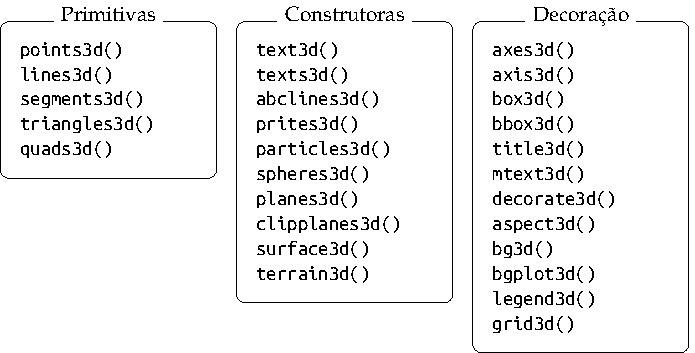
\includegraphics{./tikz/rgl-2.pdf}
}

%----------------------------------------------------------------------

\subsection{Exemplos}

\begin{frame}

  Praticando:
  \begin{enumerate}
  \item \href{run:./R/rgl/rgl.R}{R Script rgl}
  \item \href{run:./rgl/RGL.html}{Galeria rgl IGUIR}
  \end{enumerate}

  Algumas aplicações com o rgl:
  \begin{itemize}
    \itemsep1pt\parskip0pt\parsep0pt
  \item
    \href{http://cran.r-project.org/web/packages/rgl/vignettes/}{Galeria
      do autor},
  \item \href{http://www.r-bloggers.com/?s=rgl}{Busca no R Bloggers}
  \end{itemize}

\end{frame}
